\documentclass[]{book}

\usepackage{import}
\usepackage{preamble}
\usepackage{tikz}

\begin{document}

\noindent BECA / Huson / 11.1 IB Math \hspace{2in} Name:\\*
26 November 2018
\begin{center}
{\Large Classwork: Exponents and radicals}\\
\textit{Do these problems without a calculator. Use algebra properties to simplify each expression.}
\end{center}

%\vspace{0.2 cm}

\begin{enumerate}

\subsection*{Exponent rules}

\item $3x^2 \times 2x^4y^2$
\item $\displaystyle \frac{1}{2} (xy^2) \times \frac{2}{3}(x^2y)$
\item $(a^2b^3)(ab^3)$
\item $x^3 \div x^3$
\item $4y^5 \div (2y)^2$
\item $(x^5)^2$
\item $(-a^2)^3$

\subsection*{Fractional and negative exponents}

\item $\displaystyle  16^\frac{1}{2}$
\item $\displaystyle  27^\frac{1}{3}$
\item $\displaystyle  125^\frac{2}{3}$
\item $\displaystyle  (\frac{4}{9})^\frac{3}{2}$
\item $2^{-4}$
\item $9^{-\frac{3}{2}}$
\item $(\frac{27}{8})^{-\frac{4}{3}}$

\subsection*{Radicals and exponents}
Simplify, leaving no negative or fractional exponents.

\item $(9x^2)^\frac{1}{2}$
\item $\sqrt{25y^{-4}}$
\item $\displaystyle  \frac{x \sqrt{25x}}{x^{2}}$
\item $\displaystyle  \sqrt[3]{\frac{y^6}{x^{9}}}$




\newpage

\item Let $\displaystyle f(x) = \frac{1}{2}x  - 2$, for $-5 \leq x \leq 5$.
\begin{enumerate}
\item On the  grid below, sketch the graph of $f$.
\item Consider the graph of $f$ . Write down
\begin{enumerate}
\item the slope;
\item the $y$-intercept;
\item the $x$-intercept;
\end{enumerate}
\item the vertex as an ordered pair.
\begin{enumerate}
\item What is the value of $f(2)$?;
\item Plot the point on the graph representing $(2, f(2)$.;
\end{enumerate}
\end{enumerate}



\begin{figure}[!htbp]
\begin{center}
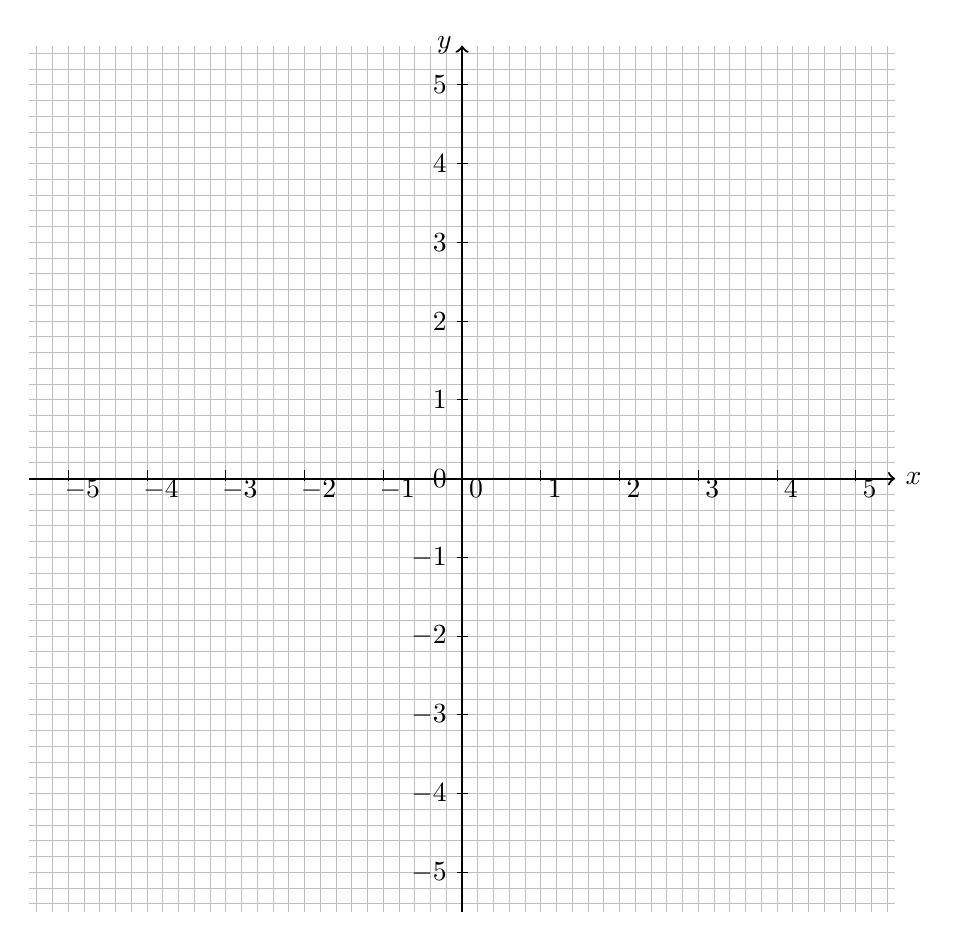
\begin{tikzpicture}

%grid
\draw [color=black,, xstep=1.0cm,ystep=1.0cm] (-5.5,-5.5) grid (5.5,5.5);
\draw [color=lightgray,, xstep=0.2cm,ystep=0.2cm] (-5.5,-5.5) grid (5.5,5.5);

\foreach \x in {-5, -4, -3, -2, -1, 0,1,2,3,4,5}
\draw[shift={(\x,0)},color=black] (0pt,-1pt) -- (0pt,3pt) node[below]  {$\quad \x$};

\foreach \y in {-5,-4,-3,-2,-1,0,1,2,3,4,5}
\draw[shift={(0,\y)},color=black] (2pt,0pt) -- (-2pt,0pt) node[left]  {$\y$};

\draw [thick, ->] (-5.5,0) -- (+5.5,0) node [right] {$x$};
\draw [thick, ->] (0,-5.5) -- (0,5.5) node [left] {$y$};

\end{tikzpicture}
\end{center}
\end{figure}

\end{enumerate}

\end{document}
